\section{Appendix A: Online Survey}
\label{appendix:A}
\noindent Survey Title: Working in Berlin without (fluent) German language skills

\subsection*{Privacy Protection Notice / Datenschutzhinweis}
\addcontentsline{toc}{subsection}{\protect\hspace*{1.5em}Privacy Protection Notice / Datenschutzhinweis}

A comprehensive privacy protection notice was provided in both English and German. The notice outlined that the survey “is part of a university research project on language requirements in Berlin’s job market. Participation is voluntary, and all responses will be anonymous and treated confidentially, in accordance with the EU General Data Protection Regulation (GDPR).” Respondents were also informed that we will collect “demographic information (e.g. age, education level, field of study) and your experiences with job searching in Berlin,” and that the results will be used “for academic purposes only and will not be shared with third parties. No personally identifying information (such as names, emails, or IP addresses) will be collected or stored.” Respondents were informed of their right to withdraw their participation at any time and that proceeding with the survey confirmed they were at least 18 years old and gave informed consent for the use of their responses in this academic study.

\subsection*{Questionnaire}
\addcontentsline{toc}{subsection}{\protect\hspace*{1.5em}Questionnaire}
\begin{enumerate}
	\item Privacy Protection Notice acceptance (Required)
	\begin{description}
		\item[Note:] Those who disagreed with the notice were unable to continue with the rest of the survey's questions
	\end{description}
	\item Gender (Required)
	\begin{enumerate}
		\item Man
		\item Woman
		\item Non-binary
		\item Prefer not to say
	\end{enumerate}
	\item Age (Required)
	\begin{enumerate}
		\item $<$ 18
		\item 18-25
		\item 26 – 35
		\item 36 – 45 
		\item $>$ 55
		\item 	Prefer not to say
	\end{enumerate}
	\item Living district (Required)
	\begin{enumerate}
		\item Mitte, Berlin (incl. Wedding) 
		\item	Friedrichshain-Kreuzberg, Berlin
		\item 	Pankow, Berlin
		\item	Charlottenburg-Wilmersdorf, Berlin
		\item	Spandau, Berlin
		\item	Steglitz-Zehlendorf, Berlin
		\item	Tempelhof-Schöneberg, Berlin
		\item	Neukölln, Berlin
		\item	Treptow-Köpenick, Berlin
		\item	Marzahn-Hellersdorf, Berlin
		\item	Lichtenberg, Berlin
		\item	Reinickendorf, Berlin
		\item	Potsdam
		\item	Brandenburg
		\item[--] Other (open-ended)
	\end{enumerate}
	\item “Which educational degree are you working towards, or have completed?”  (Required)
	\begin{enumerate}
		\item Bachelor's Degree
		\item Master's Degree
		\item Doctorate Degree
		\item[--] Other (open-ended)
	\end{enumerate}
	\item “What degree are you studying?” (Required)
	\begin{itemize}
		\item[--] (open-ended response)
	\end{itemize}
	\item “What university are you currently / have most recently studied at?” (Required)
	\begin{itemize}
		\item[--] (open-ended response)
	\end{itemize}
	\item “What industries are you looking to work for?” (Required, multi-selection)
	\begin{enumerate}
		\item Education
		\item Government
		\item Public Service
		\item IT (Information Technology)
		\item Financial
		\item Marketing
		\item Manufacturing
		\item[--] Other (open-ended)
	\end{enumerate}
	\item “What is your German language proficiency?” (Required)
	\begin{enumerate}
		\item None
		\item Beginner (A1-A2)
		\item Intermediate (B1-B2)
		\item Expert (C1-C2)
	\end{enumerate}
	\item “What is your English language proficiency?” (Required)
	\begin{enumerate}
		\item None
		\item Beginner (A1-A2)
		\item Intermediate (B1-B2)
		\item Expert (C1-C2)
	\end{enumerate}
	\item “What types of employment have you been looking for?” (Required, multi-selection)
	\begin{enumerate}
		\item Working Student (Werkstudent)
		\item Internship (Praktikum)
		\item Part-Time (Teilzeit)
		\item Full-Time (Vollzeit)
		\item[--] Other (open-ended response)
	\end{enumerate}
	\item ``Have you actively searched for a job in Berlin within the last 12 months?'' (Required)
	\begin{enumerate}
		\item Yes
		\item No
	\end{enumerate}
	\item ``On average, what percentage of job listings in your field are written in English only?'' (Required)
	\begin{enumerate}
		\item 0–25\%
		\item 26–50\%
		\item 51–75\%
		\item 76–100\%
	\end{enumerate}
	\item ``How often do job listings in your field require fluent German?'' (Required)
	\begin{enumerate}
		\item Always
		\item Often
		\item Sometimes
		\item Rarely
		\item Never
	\end{enumerate}
	\item ``Have any of your job applications been rejected because of insufficient German language skills?'' (Required)
	\begin{enumerate}
		\item Yes
		\item No
	\end{enumerate}
	\item ``Have you successfully (or previously) secured employment in Berlin without fluent German skills?'' (Required)
	\begin{enumerate}
		\item Yes
		\item No
	\end{enumerate}
	\item ``In what sector?'' (Required only if ``Yes'' selection in question 16)
	\begin{itemize}
		\item[--] (open-ended response)
	\end{itemize}
	\item ``Have you ever attended a job interview in Berlin conducted entirely in English?'' (Required)
	\begin{enumerate}
		\item Yes
		\item No
		\item I have not been invited to any interviews
	\end{enumerate}
	\item ``Before moving to Berlin, did you believe you could find a job without speaking German?'' (Required)
	\begin{enumerate}
		\item Strongly agree
		\item Agree
		\item Neutral
		\item Disagree
		\item Strongly disagree
	\end{enumerate}
	\item ``How accurate do you think this statement is: \textit{“Berlin’s reputation as an English-speaking city matches the actual job market.”}'' (Required)
	\begin{enumerate}
		\item Extremely true
		\item Somewhat true
		\item Slightly true
		\item Not true at all
	\end{enumerate}
	\item ``Do you have any other comments on your experience navigating Berlin’s job market?'' (Required)
	\begin{itemize}
		\item[--] (open-ended response)
	\end{itemize}
\end{enumerate}

\vspace{1.5em}

\subsection*{Segmentation \& Collection}
\addcontentsline{toc}{subsection}{\protect\hspace*{1.5em}Segmentation \& Collection}
\begin{itemize}
  \item The survey link and a brief explanation were sent by email or WhatsApp group message to expatriates/migrants who live or study in the Berlin Metropolitan Area.
  \item Respondents were required to sign in to a valid Microsoft account to submit the form. This was to prevent more than one response per respondent. No Microsoft account details, email addresses, or other personal information were collected except for those specifically mentioned in the questionnaire.
\end{itemize}

\subsection*{Pie Charts} \vspace{1.5em}
\addcontentsline{toc}{subsection}{\protect\hspace*{1.5em}Pie Charts}
\noindent \centering
\graphicspath{ {./attachments/appA} }
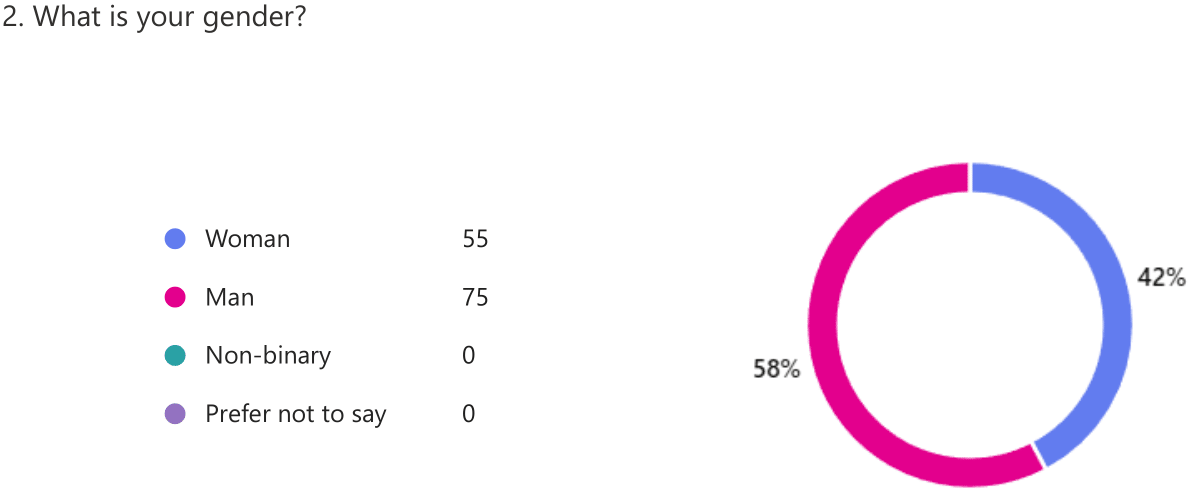
\includegraphics[width=\linewidth]{2}
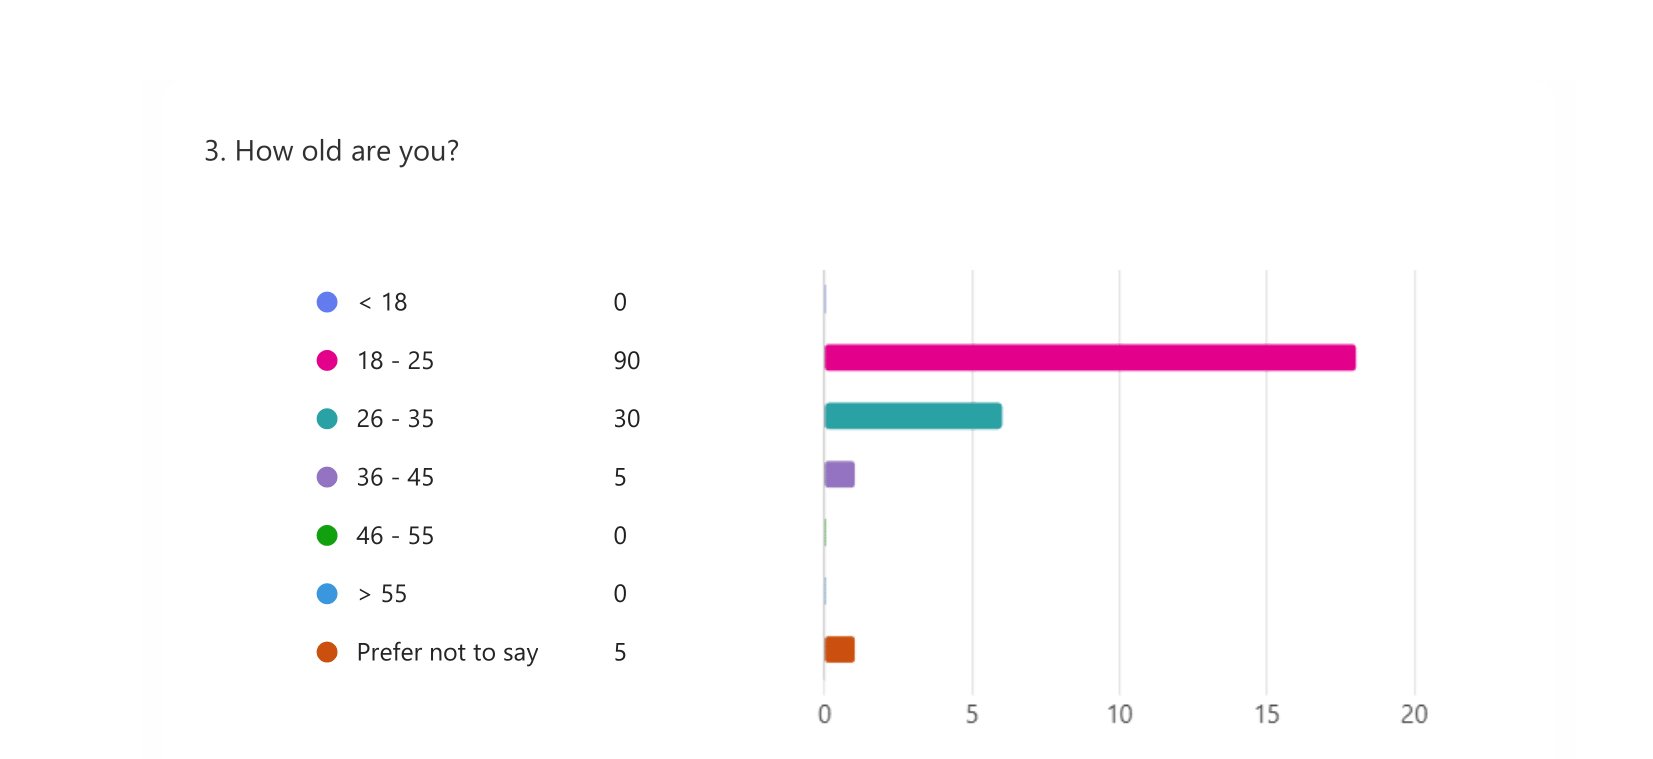
\includegraphics[width=\linewidth]{3}
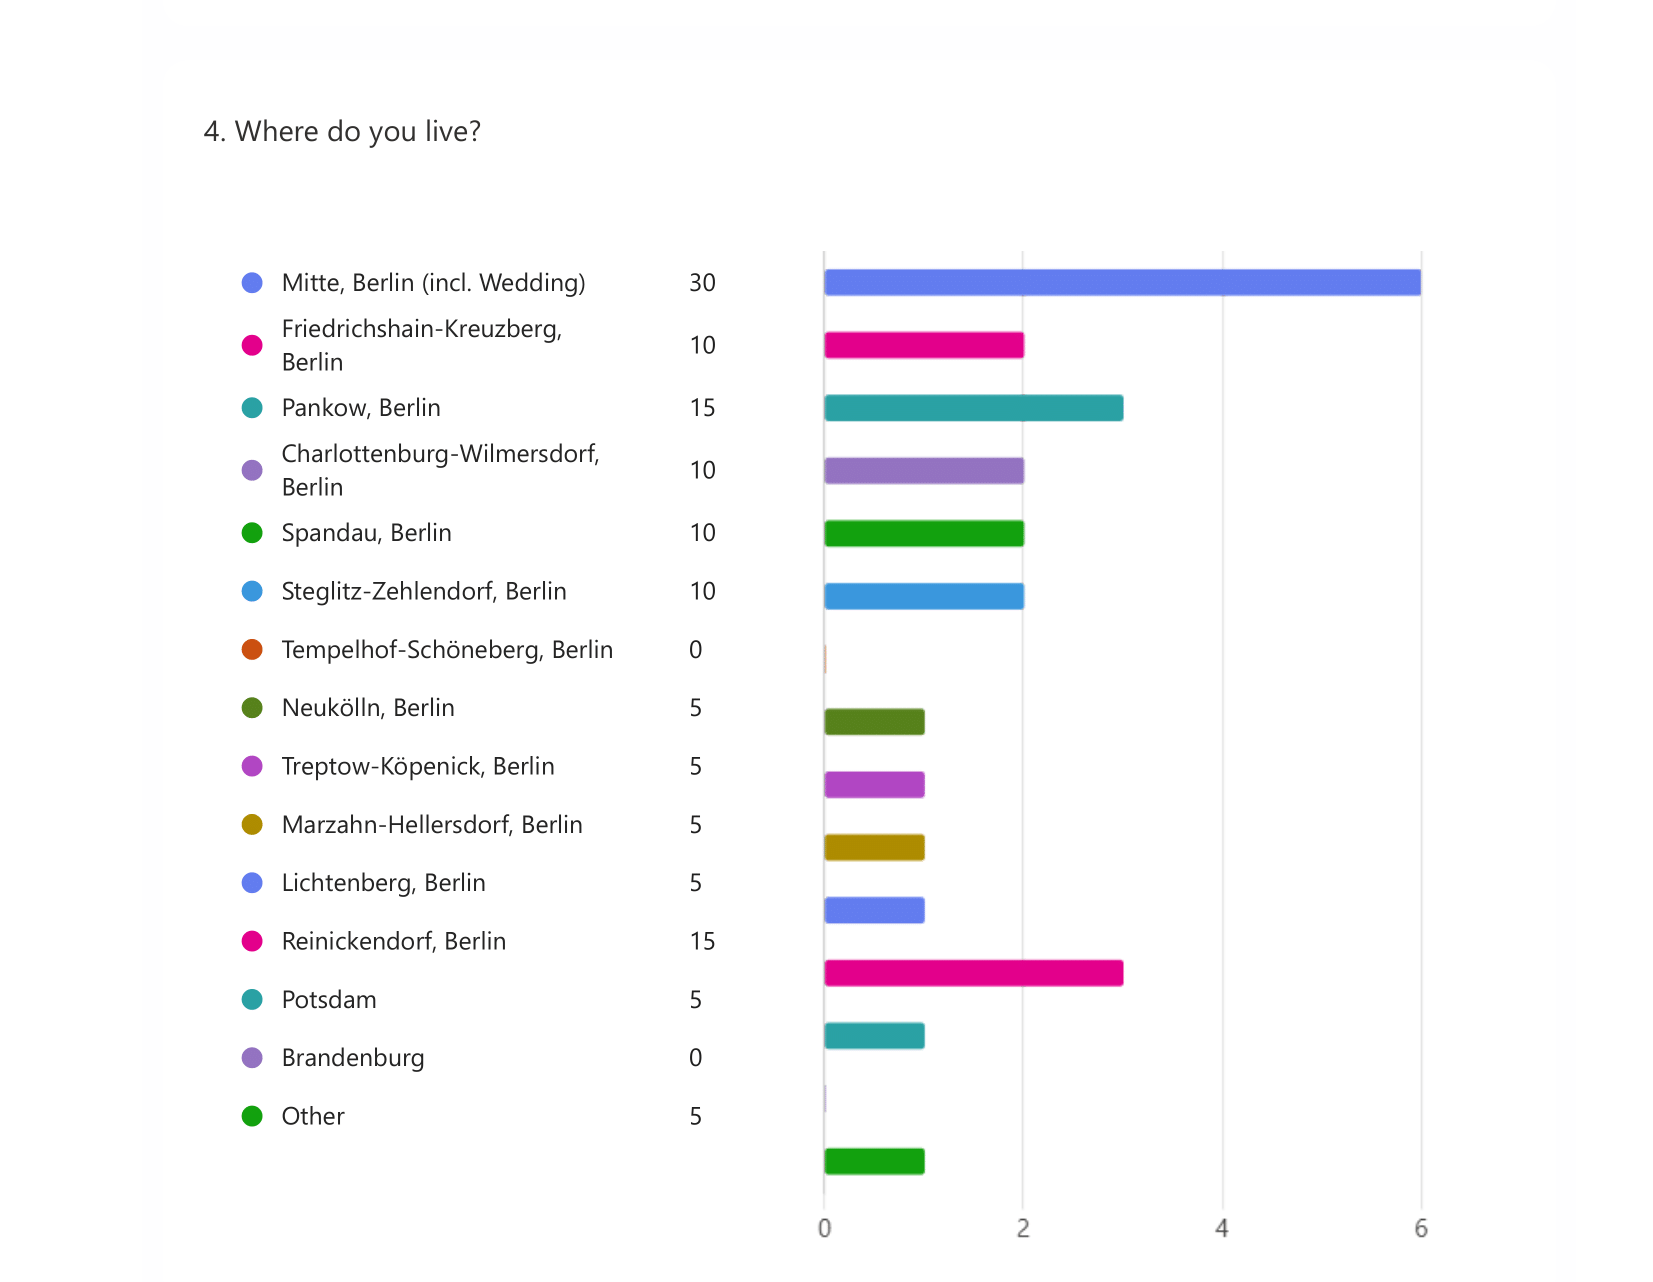
\includegraphics[width=\linewidth]{4}
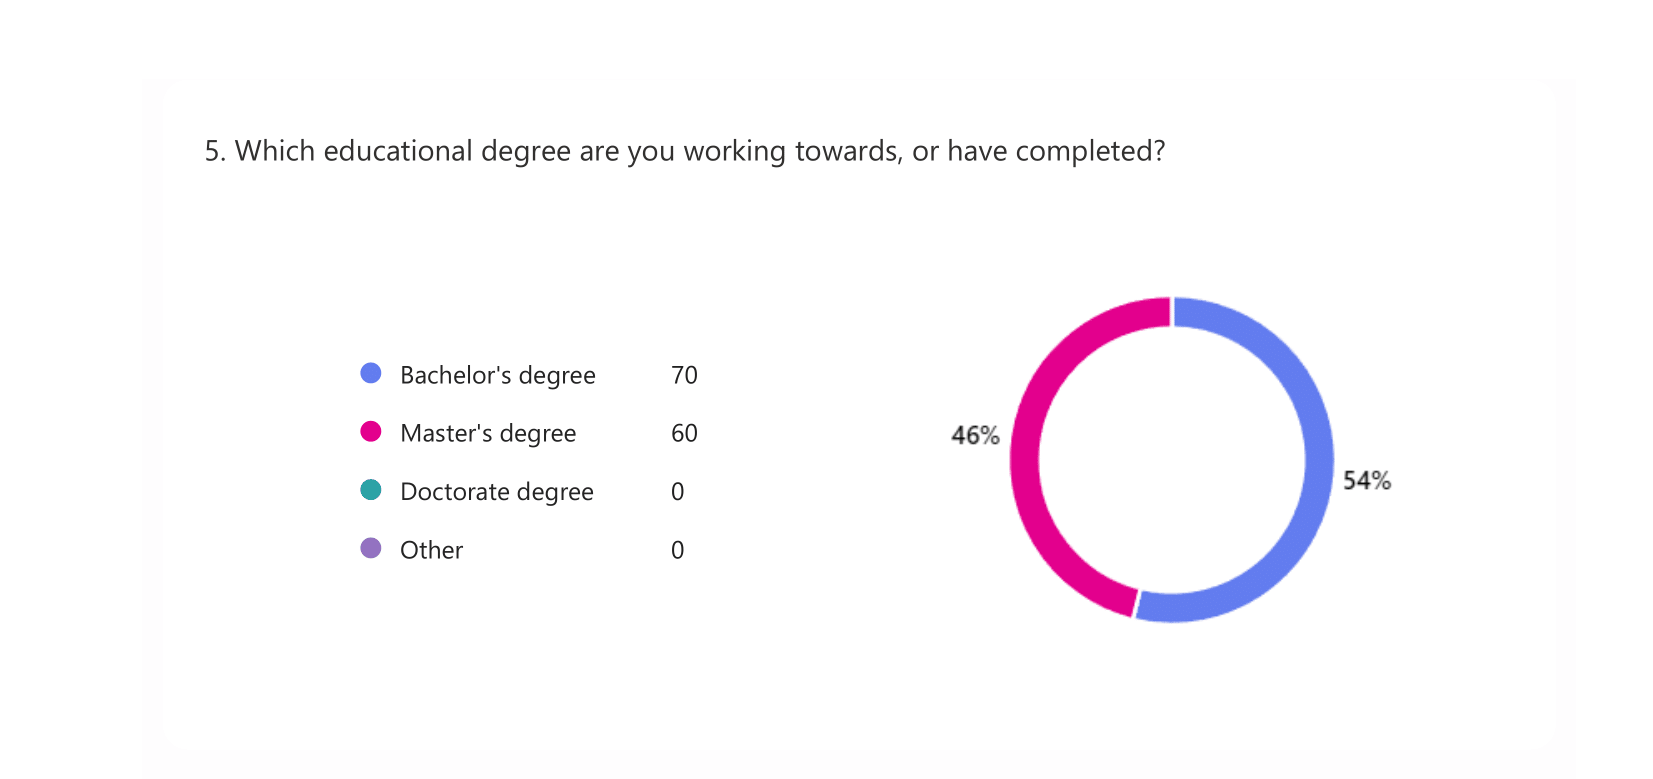
\includegraphics[width=\linewidth]{5}
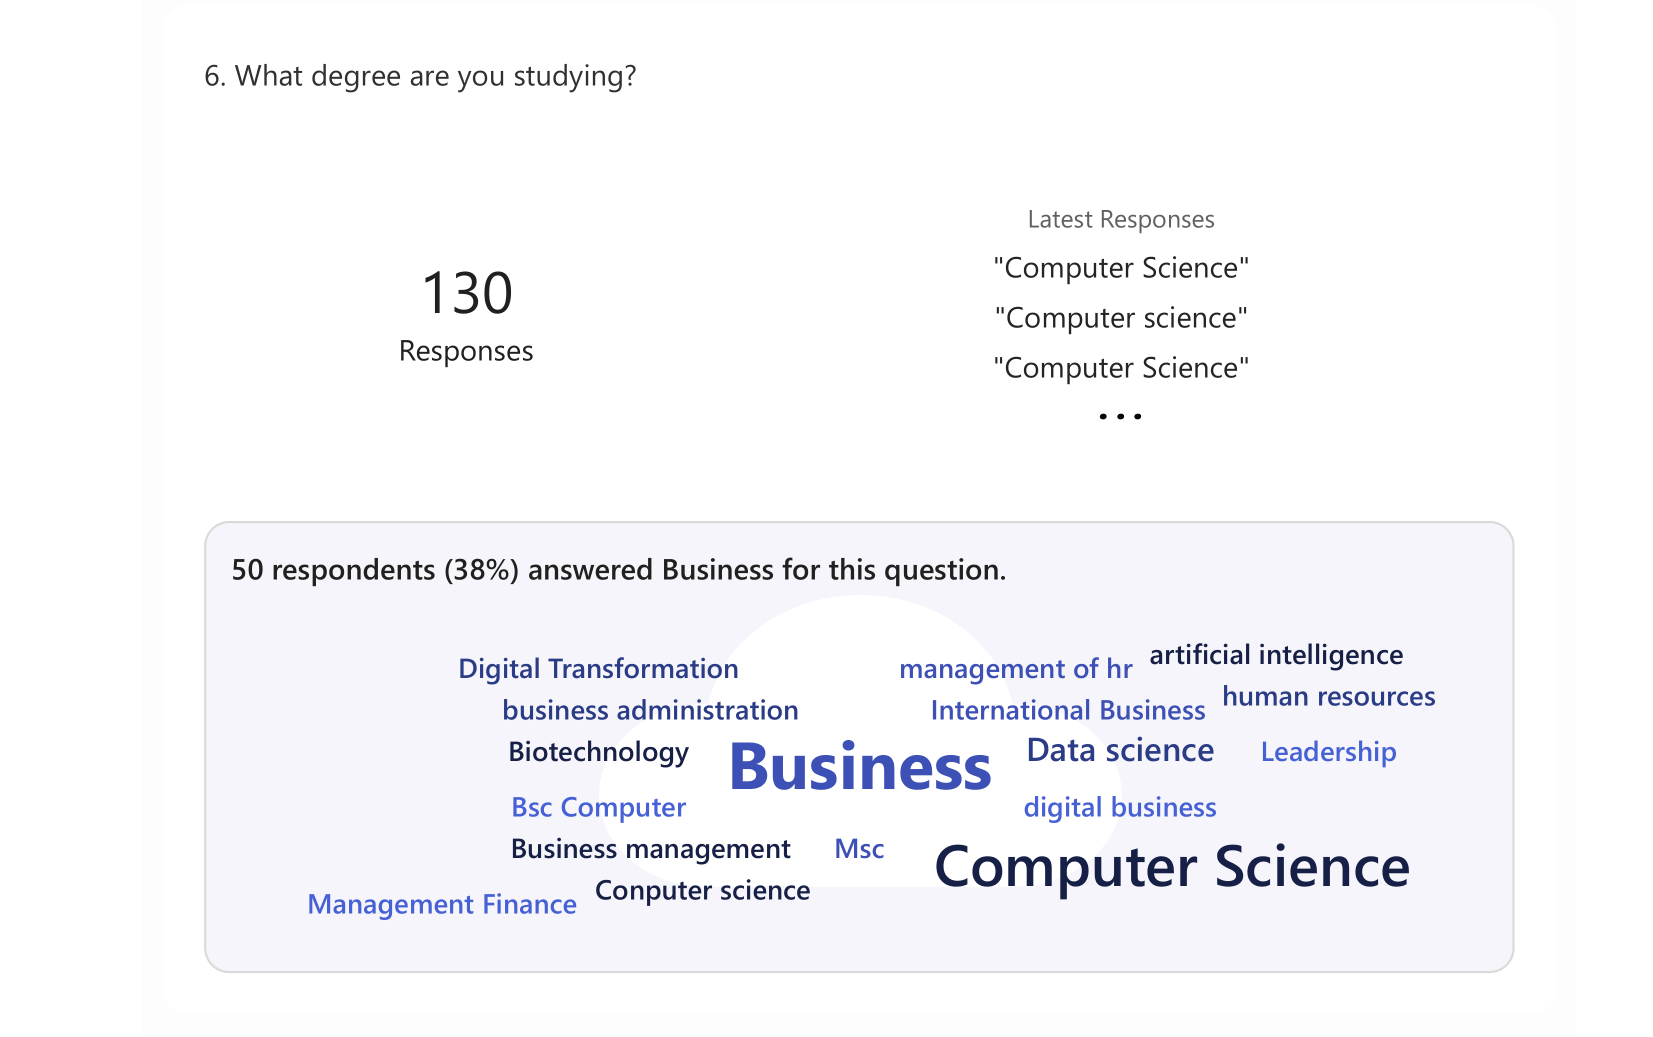
\includegraphics[width=\linewidth]{6}

\includegraphics[width=\linewidth]{7}
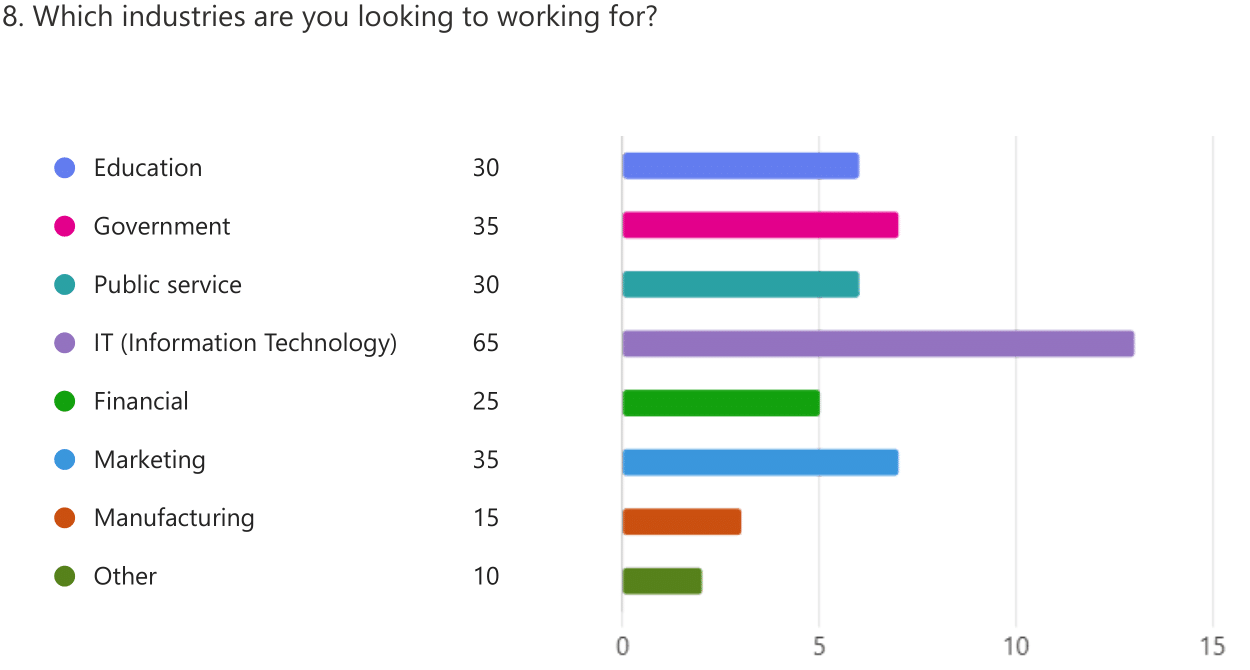
\includegraphics[width=\linewidth]{8}
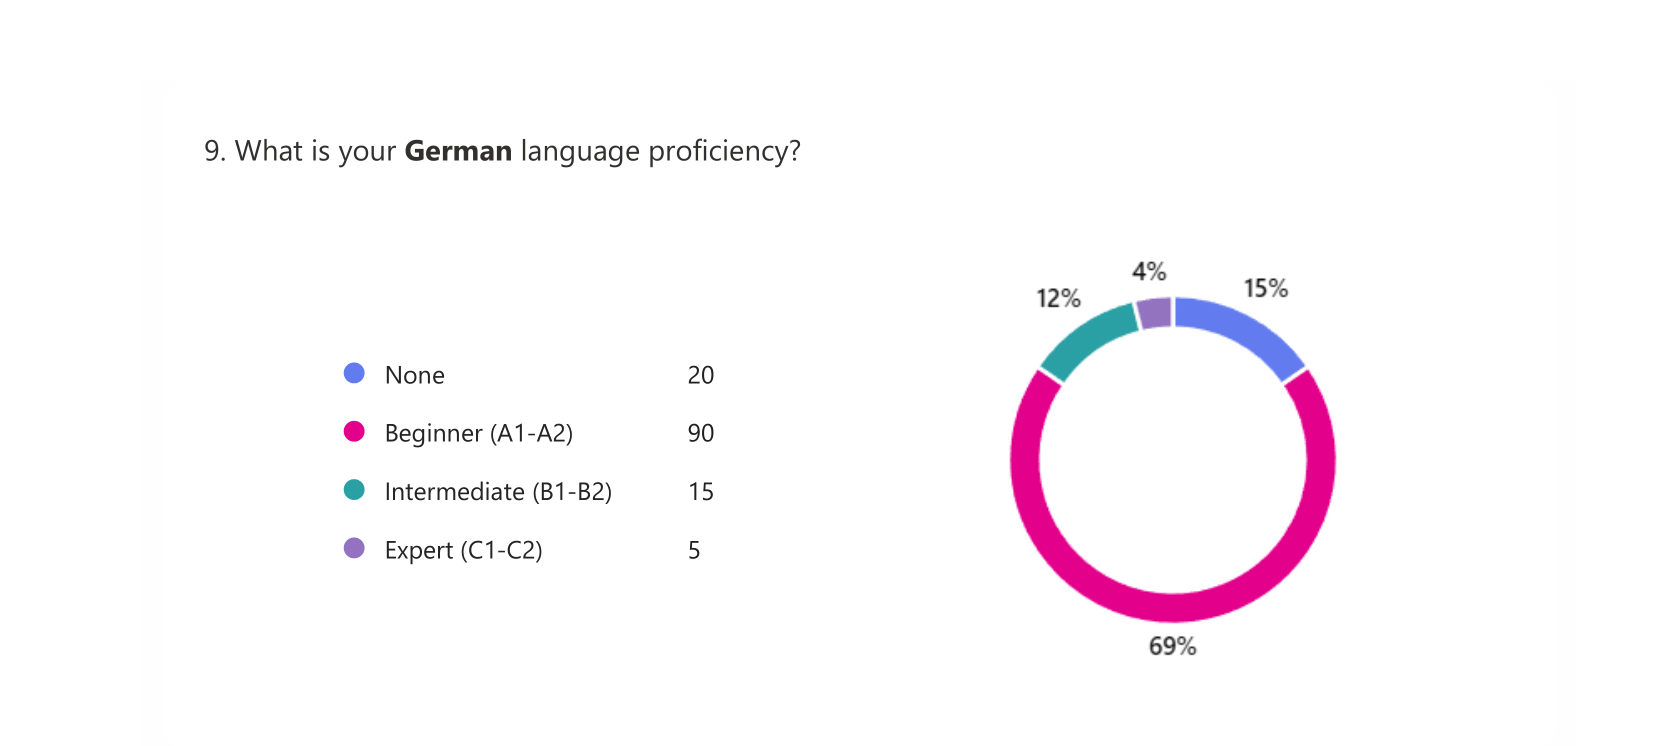
\includegraphics[width=\linewidth]{9}
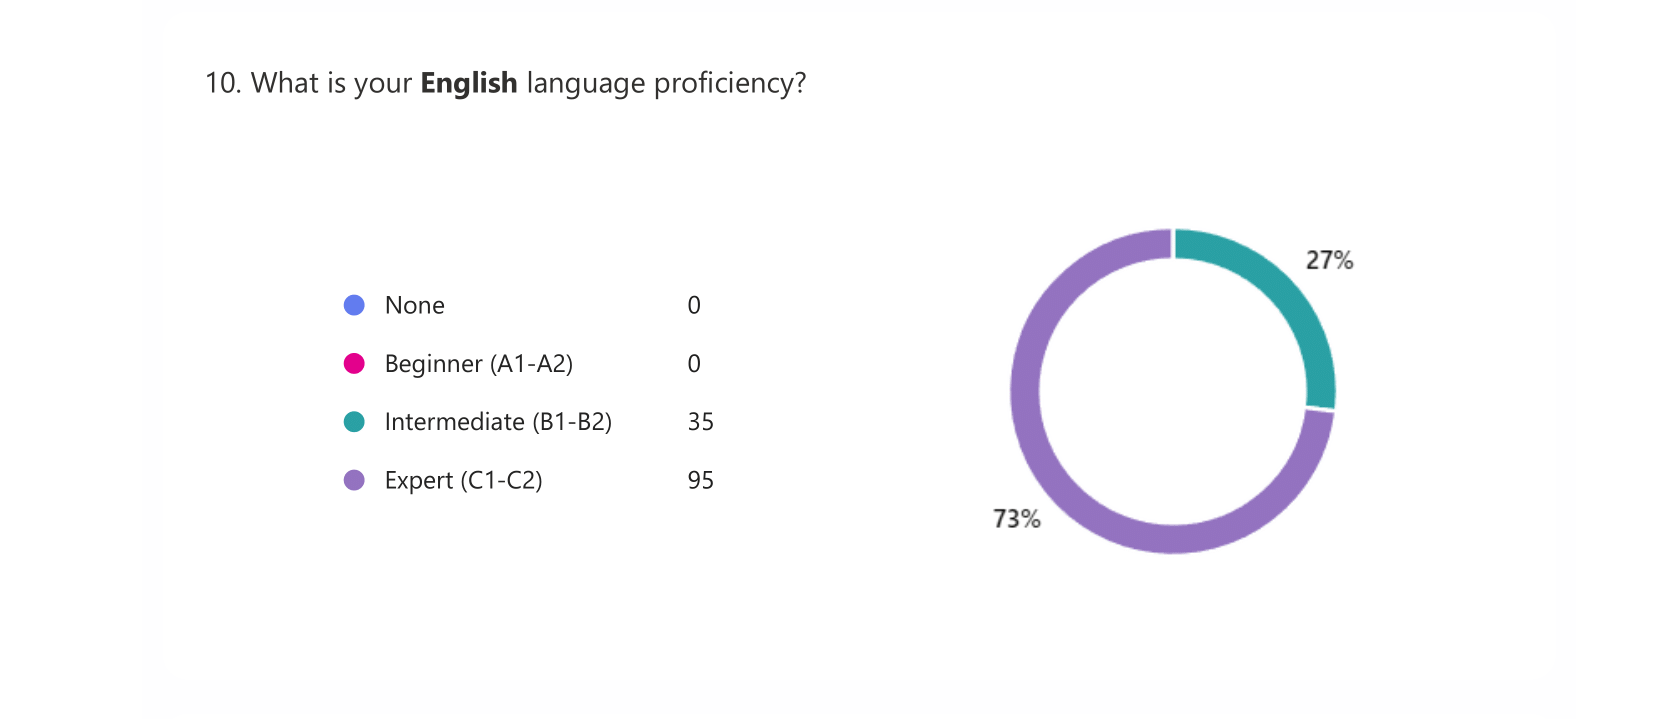
\includegraphics[width=\linewidth]{10}
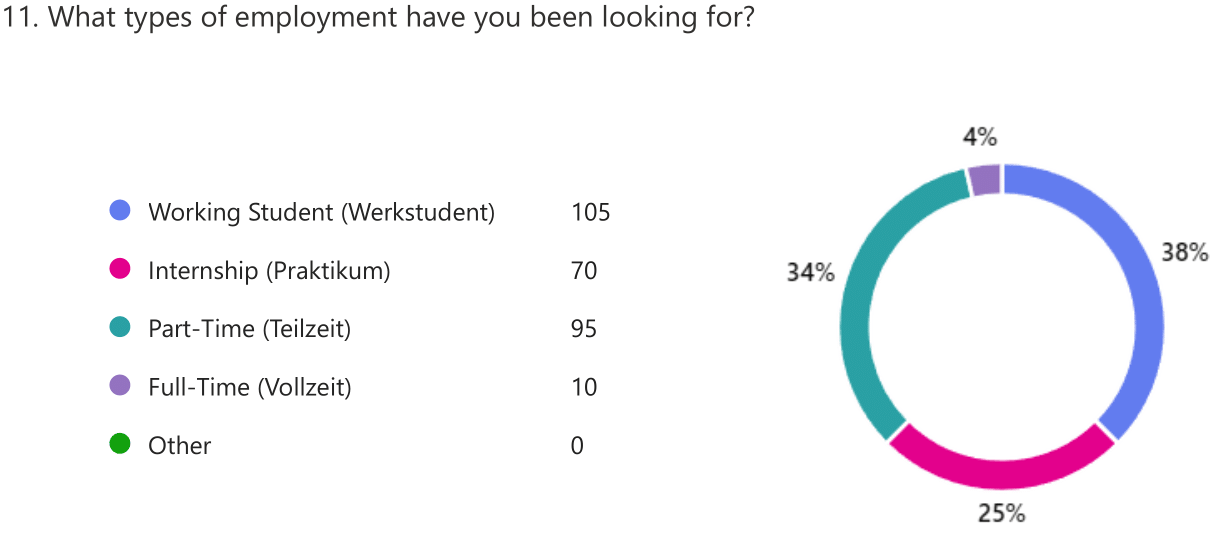
\includegraphics[width=\linewidth]{11}
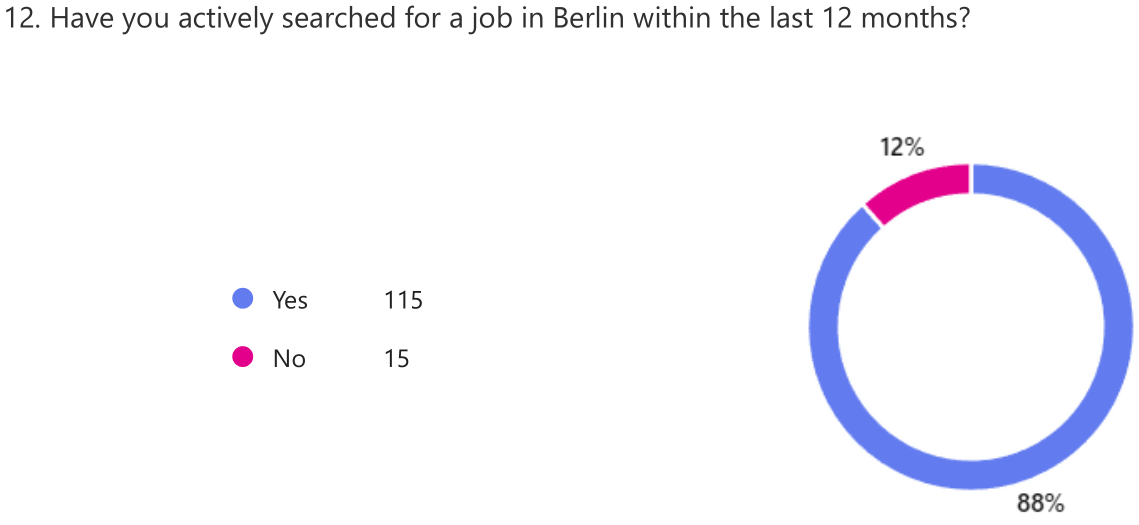
\includegraphics[width=\linewidth]{12}
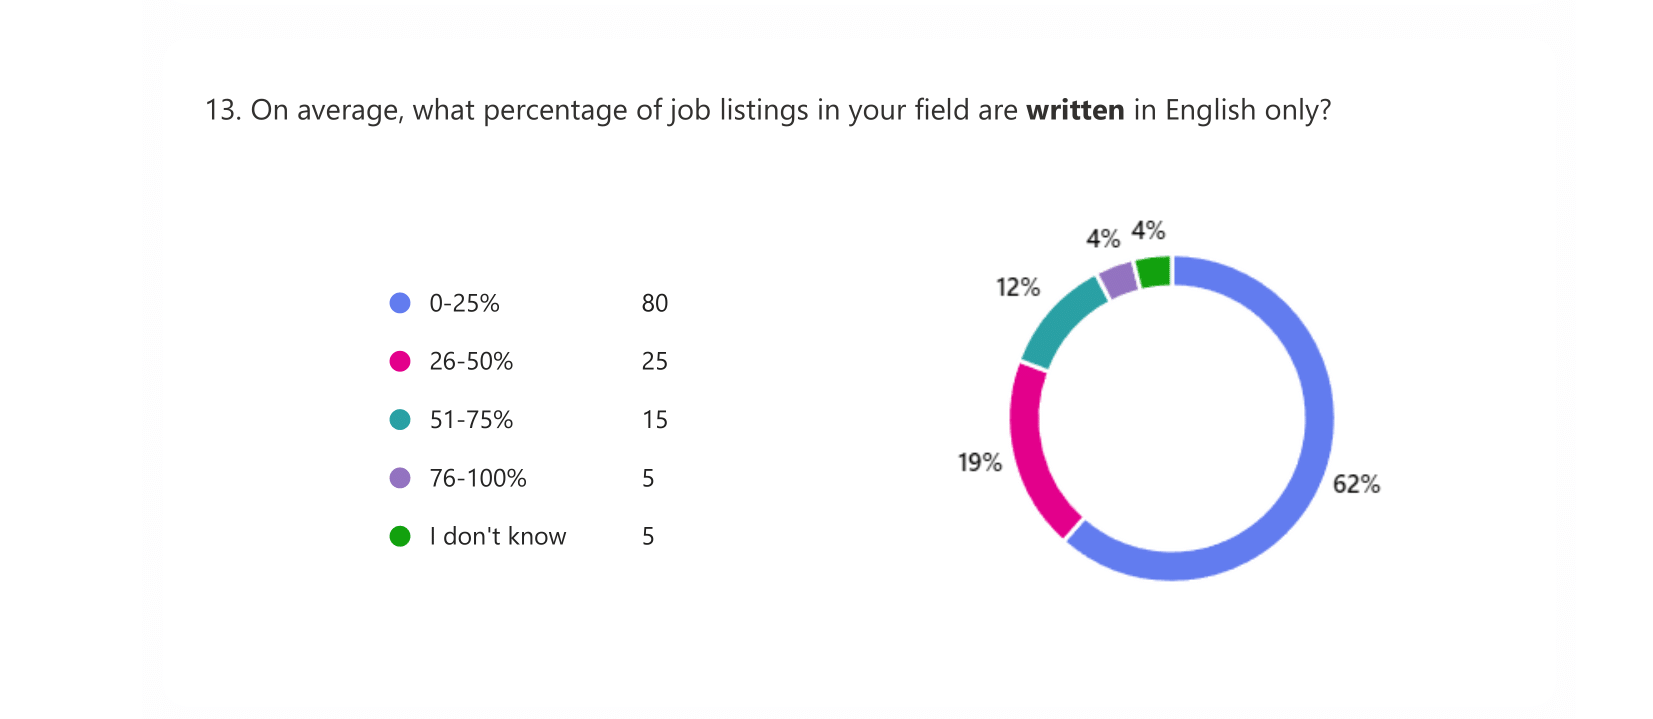
\includegraphics[width=\linewidth]{13}
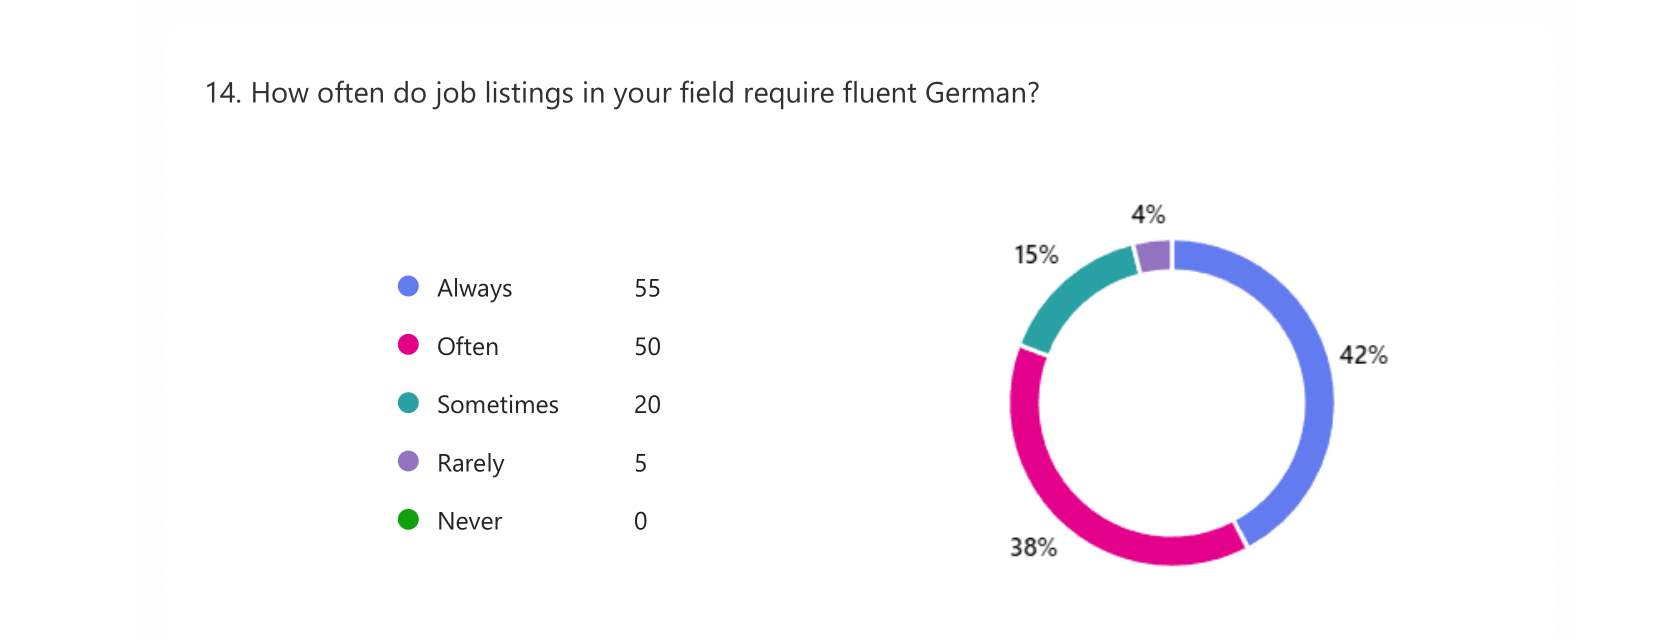
\includegraphics[width=\linewidth]{14}
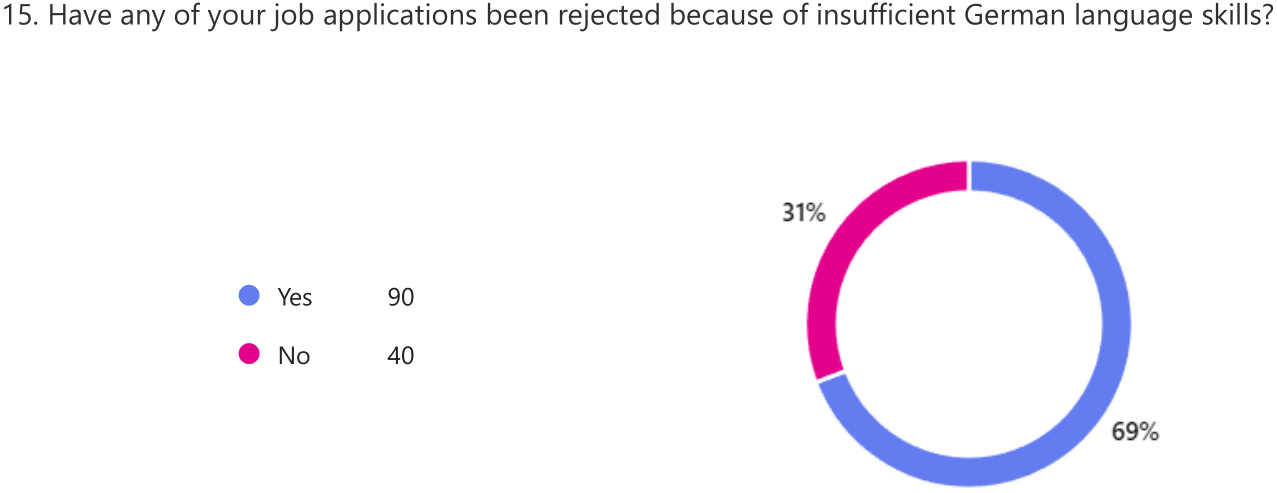
\includegraphics[width=\linewidth]{15}
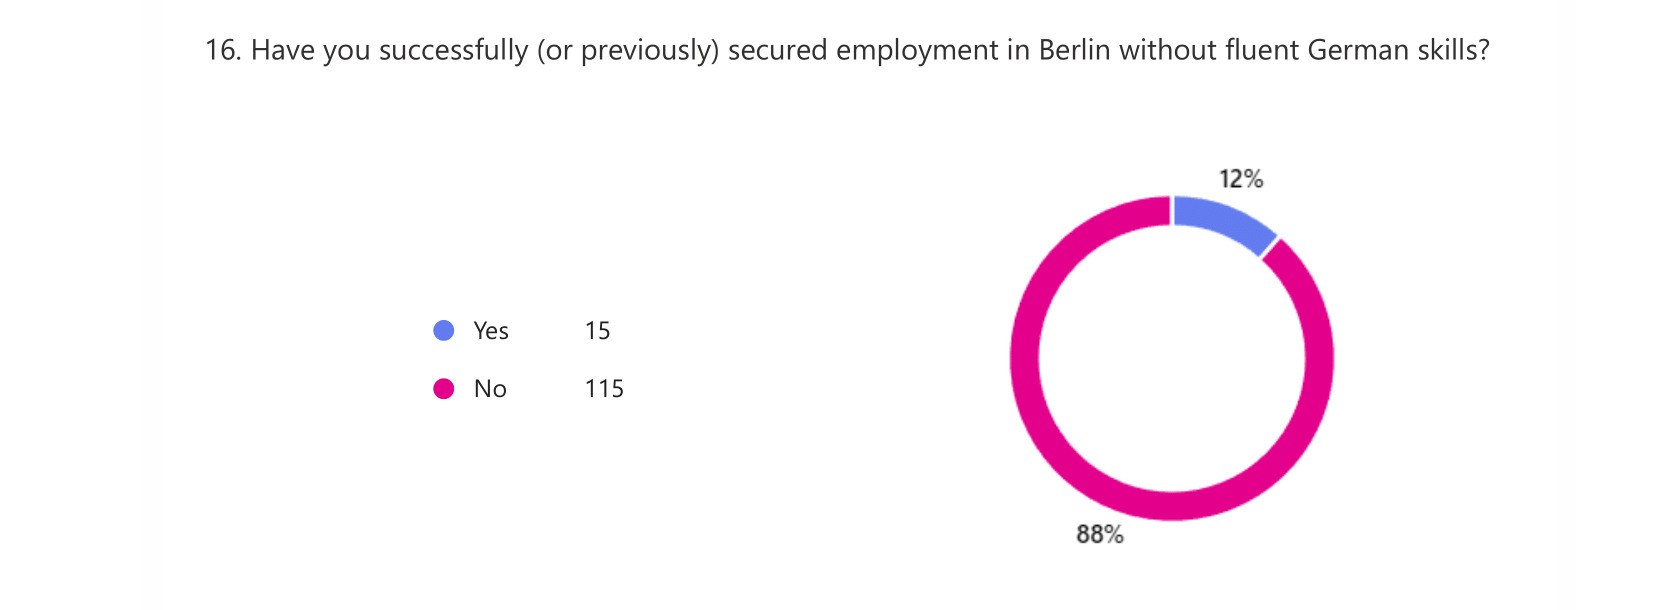
\includegraphics[width=\linewidth]{16}
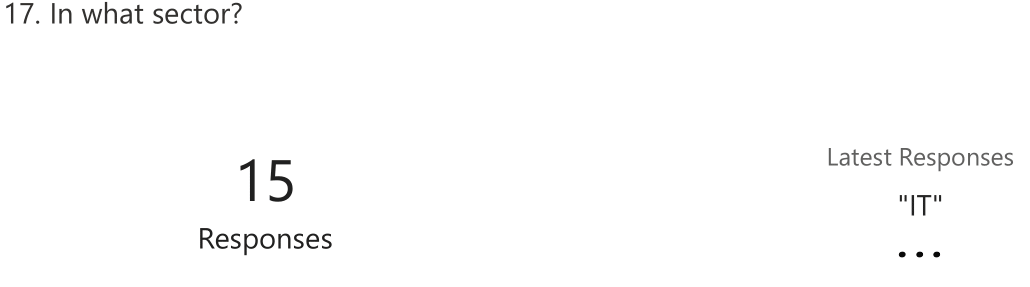
\includegraphics[width=\linewidth]{17}
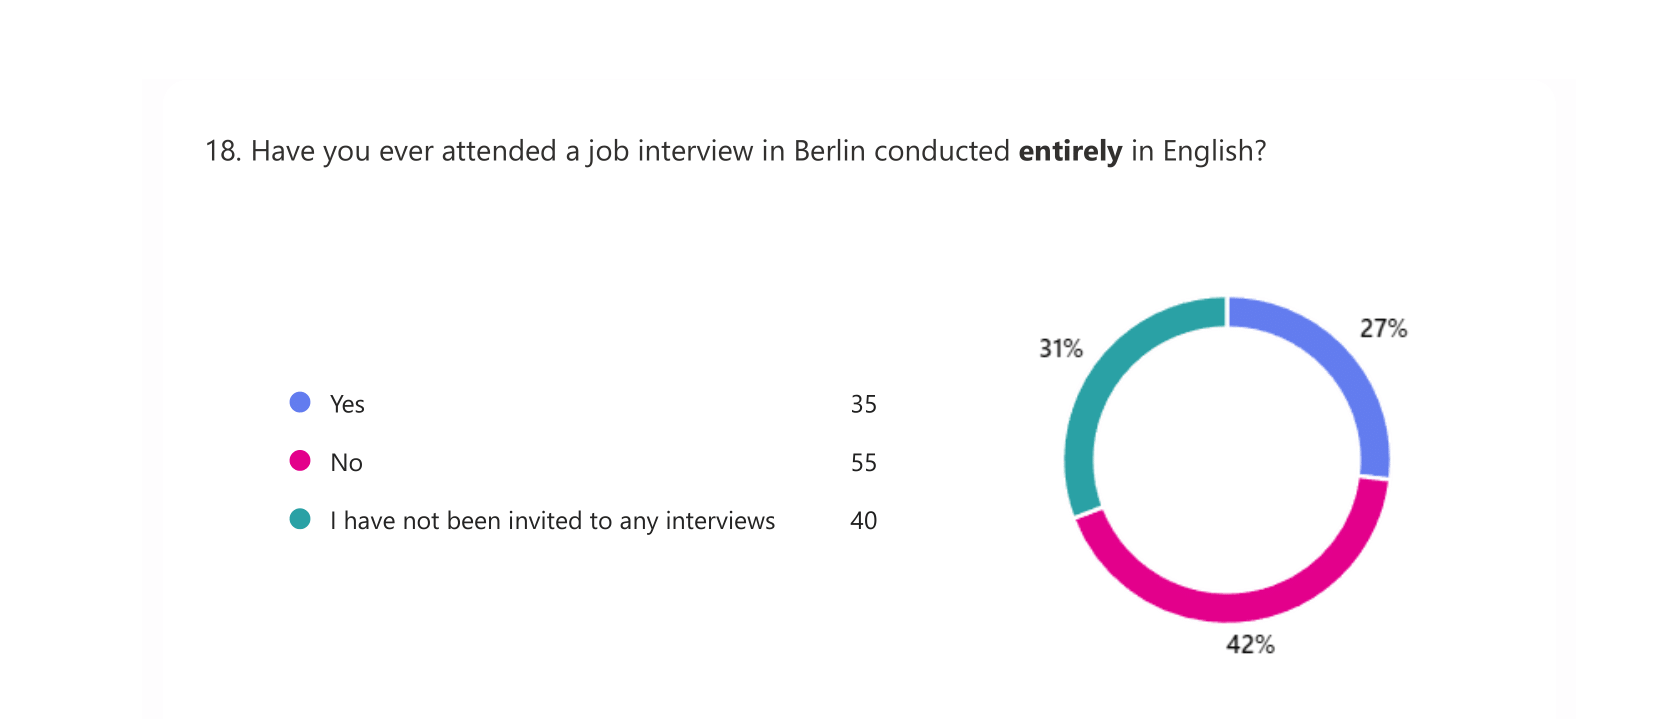
\includegraphics[width=\linewidth]{18}
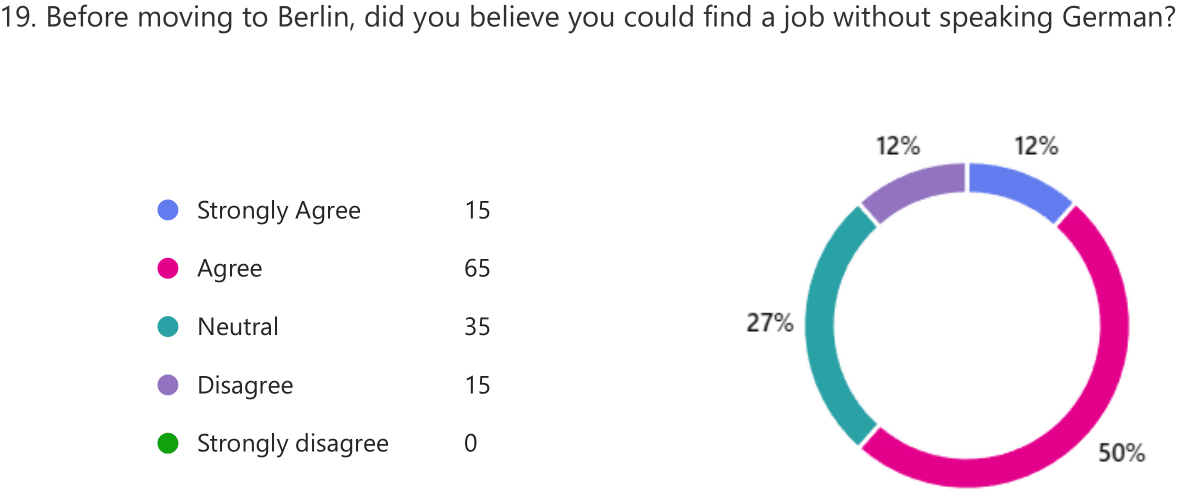
\includegraphics[width=\linewidth]{19}
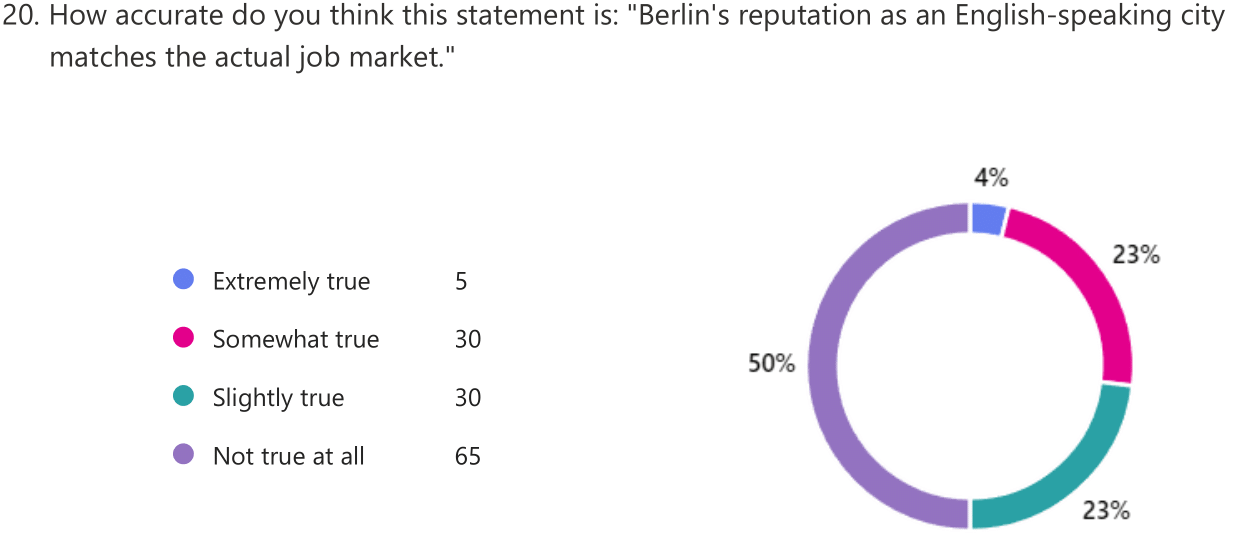
\includegraphics[width=\linewidth]{20}
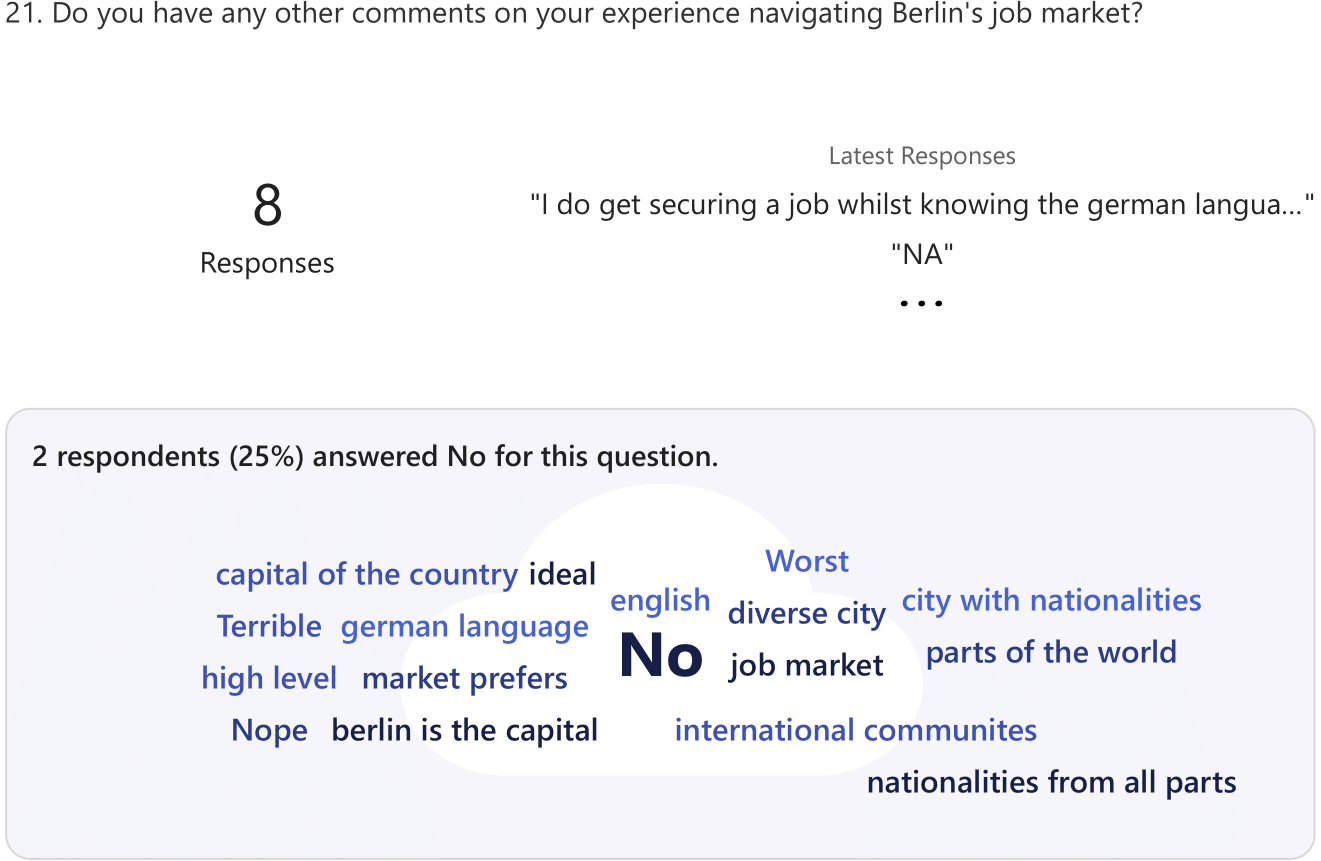
\includegraphics[width=\linewidth]{21}

\justifying
\clearpage